\documentclass{article}

\usepackage{postprocess/context/arxiv}

\usepackage[utf8]{inputenc} % allow utf-8 input
\usepackage{amsmath}
\usepackage[T1]{fontenc}    % use 8-bit T1 fonts
\usepackage{hyperref}       % hyperlinks
\usepackage{url}            % simple URL typesetting
\usepackage{booktabs}       % professional-quality tables
\usepackage{amsfonts}       % blackboard math symbols
\usepackage{nicefrac}       % compact symbols for 1/2, etc.
\usepackage{microtype}      % microtypography
\usepackage{graphicx}
\usepackage{natbib}
\usepackage{doi}
\usepackage{float}
\usepackage{subcaption}
\usepackage{wrapfig}

\title{Causal Discovery Report on Sachs}

\author{ \href{https://orcid.org/0000-0000-0000-0000}{
\includegraphics[scale=0.06]{postprocess/context/orcid.pdf}\hspace{1mm}Causal Copilot}}

\renewcommand{\headeright}{Technical Report}
\renewcommand{\undertitle}{Technical Report}

\hypersetup{
pdftitle={Causal Discovery Report on Sachs},
pdfauthor={Causal Copilot},
pdfkeywords={Causal Discovery, Large Language Model, PC, Sachs},
}

\begin{document}
\maketitle

\begin{abstract}
This study analyzes a dataset of signaling molecules and proteins relevant to cellular signaling pathways, particularly focusing on the MAPK and PI3K pathways. Utilizing a robust causal discovery methodology assisted by a large language model, we implemented data preprocessing, algorithm selection, and hyperparameter tuning before refining our causal graph through Bootstrap and expert insights. The analysis uncovered a complex web of interactions among key proteins, revealing direct influences and feedback loops, such as Mek's activation of Raf and PIP3's regulation by Plcg and PIP2. While the results indicate high confidence in certain causal relationships, the reliability analysis suggests a mixed reliability for specific edges. Overall, this study contributes to enhancing causal discovery methodologies in cellular signaling research, providing deeper insights into the intricate dynamics governing cellular processes.
\end{abstract}

\keywords{Causal Discovery, Large Language Model, PC, Sachs}

\raggedbottom
\section{Introduction}
In exploring the complex dynamics of cellular signaling pathways, this study focuses on a dataset containing key signaling molecules and proteins, including Raf, Mek, Plcg, PIP2, PIP3, Erk, Akt, PKA, PKC, P38, and Jnk. Each of these variables plays a significant role in various cellular processes, particularly within the MAPK and PI3K signaling pathways. With established causal relationships among these proteins—such as Raf activating Mek and Mek subsequently phosphorylating Erk—understanding their interconnected roles is essential for deciphering the intricate networks of cellular signaling. Moreover, insights into feedback mechanisms, temporal dynamics, and experimental data collection are crucial for accurately determining causality in this biological context. This report aims to leverage both the variable interactions and domain-specific knowledge to enhance causal discovery methodologies and contribute to a deeper understanding of cellular behavior.

\section{Background Knowledge}
\subsection{Detailed Explanation about the Variables}
\begin{itemize}
    \item \textbf{Raf (Rapidly Accelerated Fibrosarcoma)}: A serine/threonine kinase that plays a key role in the MAPK signaling pathway. It is activated by RAS proteins and subsequently activates MEK. Raf functions as a pivotal player in transducing signals related to growth and proliferation, influencing various downstream responses in cellular contexts.
    
    \item \textbf{Mek (Mitogen-activated protein kinase/extracellular signal-regulated kinase kinase)}: A dual-specificity kinase that is activated by Raf and, in turn, phosphorylates ERK. Mek is critical for the propagation of the MAPK signaling cascade and is instrumental in cellular responses to growth factors.
    
    \item \textbf{Plcg (Phospholipase C-gamma)}: An enzyme involved in the hydrolysis of phosphatidylinositol 4,5-bisphosphate, resulting in the production of inositol trisphosphate and diacylglycerol, which are important second messengers in signaling cascades. It helps mediate intracellular calcium levels and activates protein kinase C.
    
    \item \textbf{PIP2 (Phosphatidylinositol 4,5-bisphosphate)}: A phospholipid that serves as a substrate for phospholipase C and is a critical component in cellular signaling and membrane dynamics. PIP2 is involved in the recruitment of various signaling proteins to membranes and plays a role in regulating cytoskeletal dynamics.
    
    \item \textbf{PIP3 (Phosphatidylinositol 3,4,5-trisphosphate)}: A product of the phosphorylation of PIP2 by PI3-kinases; it acts as a crucial second messenger in cellular signaling pathways and is particularly important for the activation of Akt, influencing processes such as cell survival, growth, and metabolism.
    
    \item \textbf{Erk (Extracellular signal-regulated kinase)}: A major component of the MAPK signaling pathway, Erk mediates a variety of cellular processes, including proliferation, differentiation, and survival. Its activation is tightly regulated and allows cells to respond to extracellular signals effectively.
    
    \item \textbf{Akt (Protein Kinase B)}: A serine/threonine-specific protein kinase that plays a pivotal role in multiple cellular processes including glucose metabolism, apoptosis, cell proliferation, and transcription. Akt is activated through PIP3 and is central to the PI3K pathway.
    
    \item \textbf{PKA (Protein Kinase A)}: Also known as cyclic AMP-dependent protein kinase, PKA is activated by cyclic AMP and participates in various signaling pathways, including those that regulate gene expression and metabolic processes. PKA is essential for mediating the effects of hormones like adrenaline.
    
    \item \textbf{PKC (Protein Kinase C)}: A family of serine/threonine kinases involved in numerous signaling processes within the cell. PKC isoforms are activated by diacylglycerol and calcium ions and play roles in growth factor signaling, cellular proliferation, and differentiation.
    
    \item \textbf{P38 (p38 MAP Kinase)}: A stress-activated protein kinase that is part of the MAPK signaling pathway. It is involved in responses to cellular stress, inflammation, and apoptosis, acting as a critical mediator in the stress response pathways.
    
    \item \textbf{Jnk (c-Jun N-terminal kinase)}: Another MAPK family member that is activated by various stress stimuli. Jnk plays a significant role in regulating the cell cycle, apoptosis, and inflammatory responses, providing a critical link between stress signals and cellular outcomes.
\end{itemize}

This dataset represents a complex network of signaling molecules whose interconnections are vital for understanding cell signaling, proliferation, and stress responses. Each variable is integral to cellular function and contributes to multiple signaling pathways, highlighting the importance of context in analyzing causal relations. Understanding the roles and interactions of these variables is essential for effective causal discovery.

\subsection{Possible Causal Relations among these Variables}

\begin{minipage}[t]{0.7\linewidth}
\begin{itemize}
    \item \textbf{Raf $\rightarrow$ Mek}: Raf activates Mek through phosphorylation, initiating the MAPK signaling cascade.  
    \item \textbf{Mek $\rightarrow$ Erk}: Mek activates Erk through phosphorylation, continuing the MAPK signaling cascade.  
    \item \textbf{Plcg $\rightarrow$ PIP2}: Plcg is responsible for hydrolyzing phosphatidylinositol 4,5-bisphosphate, leading to various downstream signaling effects.  
    \item \textbf{PIP2 $\rightarrow$ PIP3}: PIP2 is converted to PIP3 by the action of PI3-kinases, which is essential for Akt activation.  
    \item \textbf{PIP3 $\rightarrow$ Akt}: PIP3 recruits Akt to the plasma membrane, where it becomes activated and participates in various signaling pathways.  
    \item \textbf{Akt $\rightarrow$ PKA}: Akt can activate PKA by modulating cyclic AMP levels or through other signaling intermediates, influencing various cellular processes.  
    \item \textbf{PKC $\rightarrow$ P38}: PKC can activate P38 MAPK as part of stress response pathways, impacting cellular responses to environmental stimuli.  
    \item \textbf{PKC $\rightarrow$ Jnk}: PKC also has the potential to activate Jnk, which is involved in stress, apoptosis, and cell cycle regulation.  
    \item \textbf{Raf $\rightarrow$ Plcg}: Raf may enhance the activity of Plcg, linking MAPK signaling to phospholipase activation.  
    \item \textbf{Erk $\rightarrow$ PKA}: Erk can phosphorylate and activate PKA directly in signaling pathways that regulate cell metabolism and gene expression.  
    \item \textbf{Mek $\rightarrow$ P38}: Mek can also activate P38 MAPK through the MAPK signaling pathway, contributing to stress responses.  
    \item \textbf{Erk $\rightarrow$ Jnk}: Erk may influence Jnk activation indirectly via feedback loops and intersection of signaling pathways.
\end{itemize}
\end{minipage}
\hspace{0.05\textwidth}
\begin{minipage}[t]{0.3\linewidth}
    \begin{figure}[H]
        \centering
        \resizebox{\linewidth}{!}{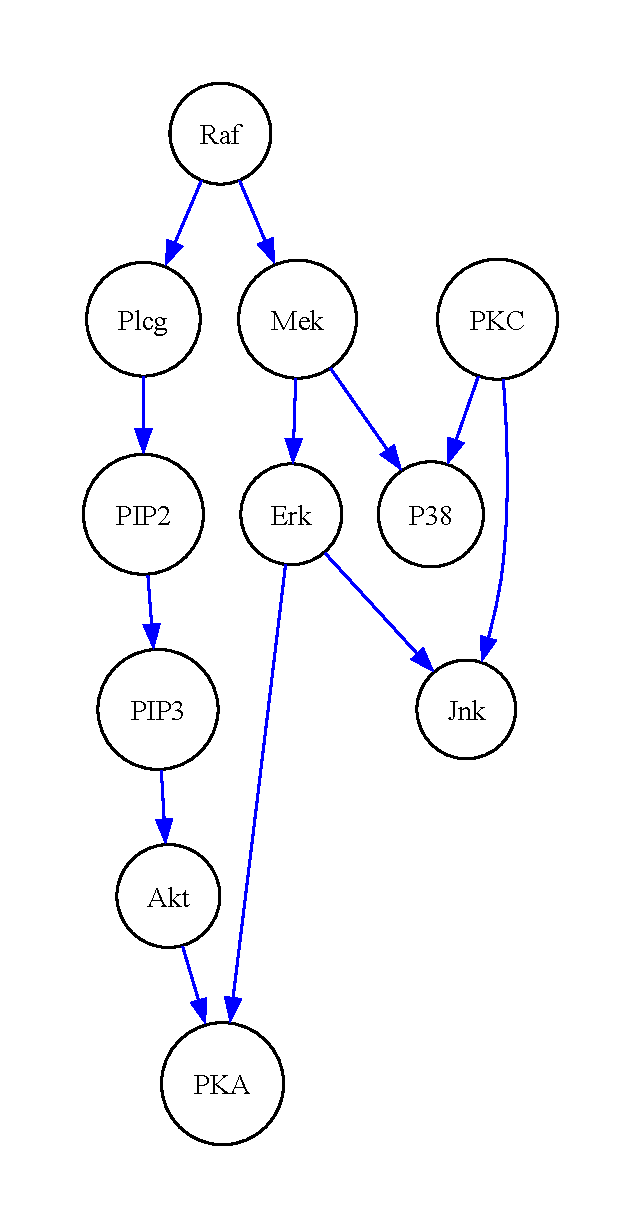
\includegraphics[height=0.3\textheight]{./demo_data/20241104_133008/sachs/output_graph/potential_relation.pdf}}
        \caption{\label{fig:relation}Possible Causal Relation Graph}
    \end{figure}
\end{minipage}

\section{Dataset Descriptions and EDA}
The following is a preview of our original dataset.

\begin{table}[H]
    \centering
    \caption{Dataset Preview}

    \resizebox{\textwidth}{!}{
        \begin{tabular}{rrrrrrrrrrr}
            \toprule
             Raf &  Mek &  Plcg &  PIP2 &  PIP3 &   Erk &  Akt &   PKA &   PKC &  P38 &  Jnk \\
            \midrule
            26.4 & 13.2 &  8.82 & 18.30 & 58.80 &  6.61 & 17.0 & 414.0 & 17.00 & 44.9 & 40.0 \\
            35.9 & 16.5 & 12.30 & 16.80 &  8.13 & 18.60 & 32.5 & 352.0 &  3.37 & 16.5 & 61.5 \\
            59.4 & 44.1 & 14.60 & 10.20 & 13.00 & 14.90 & 32.5 & 403.0 & 11.40 & 31.9 & 19.5 \\
            73.0 & 82.8 & 23.10 & 13.50 &  1.29 &  5.83 & 11.8 & 528.0 & 13.70 & 28.6 & 23.1 \\
            33.7 & 19.8 &  5.19 &  9.73 & 24.80 & 21.10 & 46.1 & 305.0 &  4.66 & 25.7 & 81.3 \\
            \bottomrule
        \end{tabular}
    }
                
\end{table}

\subsection{Data Properties}
We employ several statistical methods to identify data properties.

The shape of the data, data types, and missing values are assessed directly from the dataframe. Linearity is evaluated using Ramsey’s RESET test, followed by the Benjamini \& Yekutieli procedure for multiple test correction. Gaussian noise is assessed through the Shapiro-Wilk test, also applying the Benjamini \& Yekutieli procedure for multiple test correction. Time-Series and Heterogeneity are derived from user queries.

Properties of the dataset we analyzed are listed below.

\begin{table}[H]
    \centering
    \caption{Data Properties}

        \begin{tabular}{rrrrrrr}
            \toprule
            Shape ($n$ x $d$) & Data Type & Missing Value & Linearity & Gaussian Errors & Time-Series & Heterogeneity  \\
            \midrule
            (853, 11)   & Continuous & False & False & False & False & False \\
            \bottomrule
        \end{tabular}
        
\end{table}

\subsection{Distribution Analysis}
The following figure shows distributions of different variables. The orange dash line represents the mean, 
and the black line represents the median. Variables are categorized into three types according to their distribution characteristics.

\begin{figure}[H]
\centering
\includegraphics[width=\linewidth]{./demo_data/20241104_133008/sachs/output_graph/eda_dist.jpg}
\caption{\label{fig:dist}Distribution Plots of Variables}
\end{figure}

\begin{itemize}
\item Slight left skew distributed variables: None
\item Slight right skew distributed variables: Raf, Mek, Plcg, PIP2, PIP3, Erk, Akt, PKA, PKC, P38, Jnk
\item Symmetric distributed variables: None
\end{itemize}

\subsection{Correlation Analysis}

\begin{minipage}[t]{0.5\linewidth}
    In this analysis, we will categorize the correlation statistics of features in the dataset into three distinct categories: Strong correlations, Moderate correlations, and Weak correlations.

\begin{itemize}
\item Strong Correlated Variables: Akt and Erk
\item Moderate Correlated Variables: Mek and Raf, P38 and PKC
\item Weak Correlated Variables: None
\end{itemize}
\vfill
\end{minipage}
\hfill
\begin{minipage}[t]{0.5\linewidth}
    \begin{figure}[H]
        \centering
        \vspace{-1.5cm}
        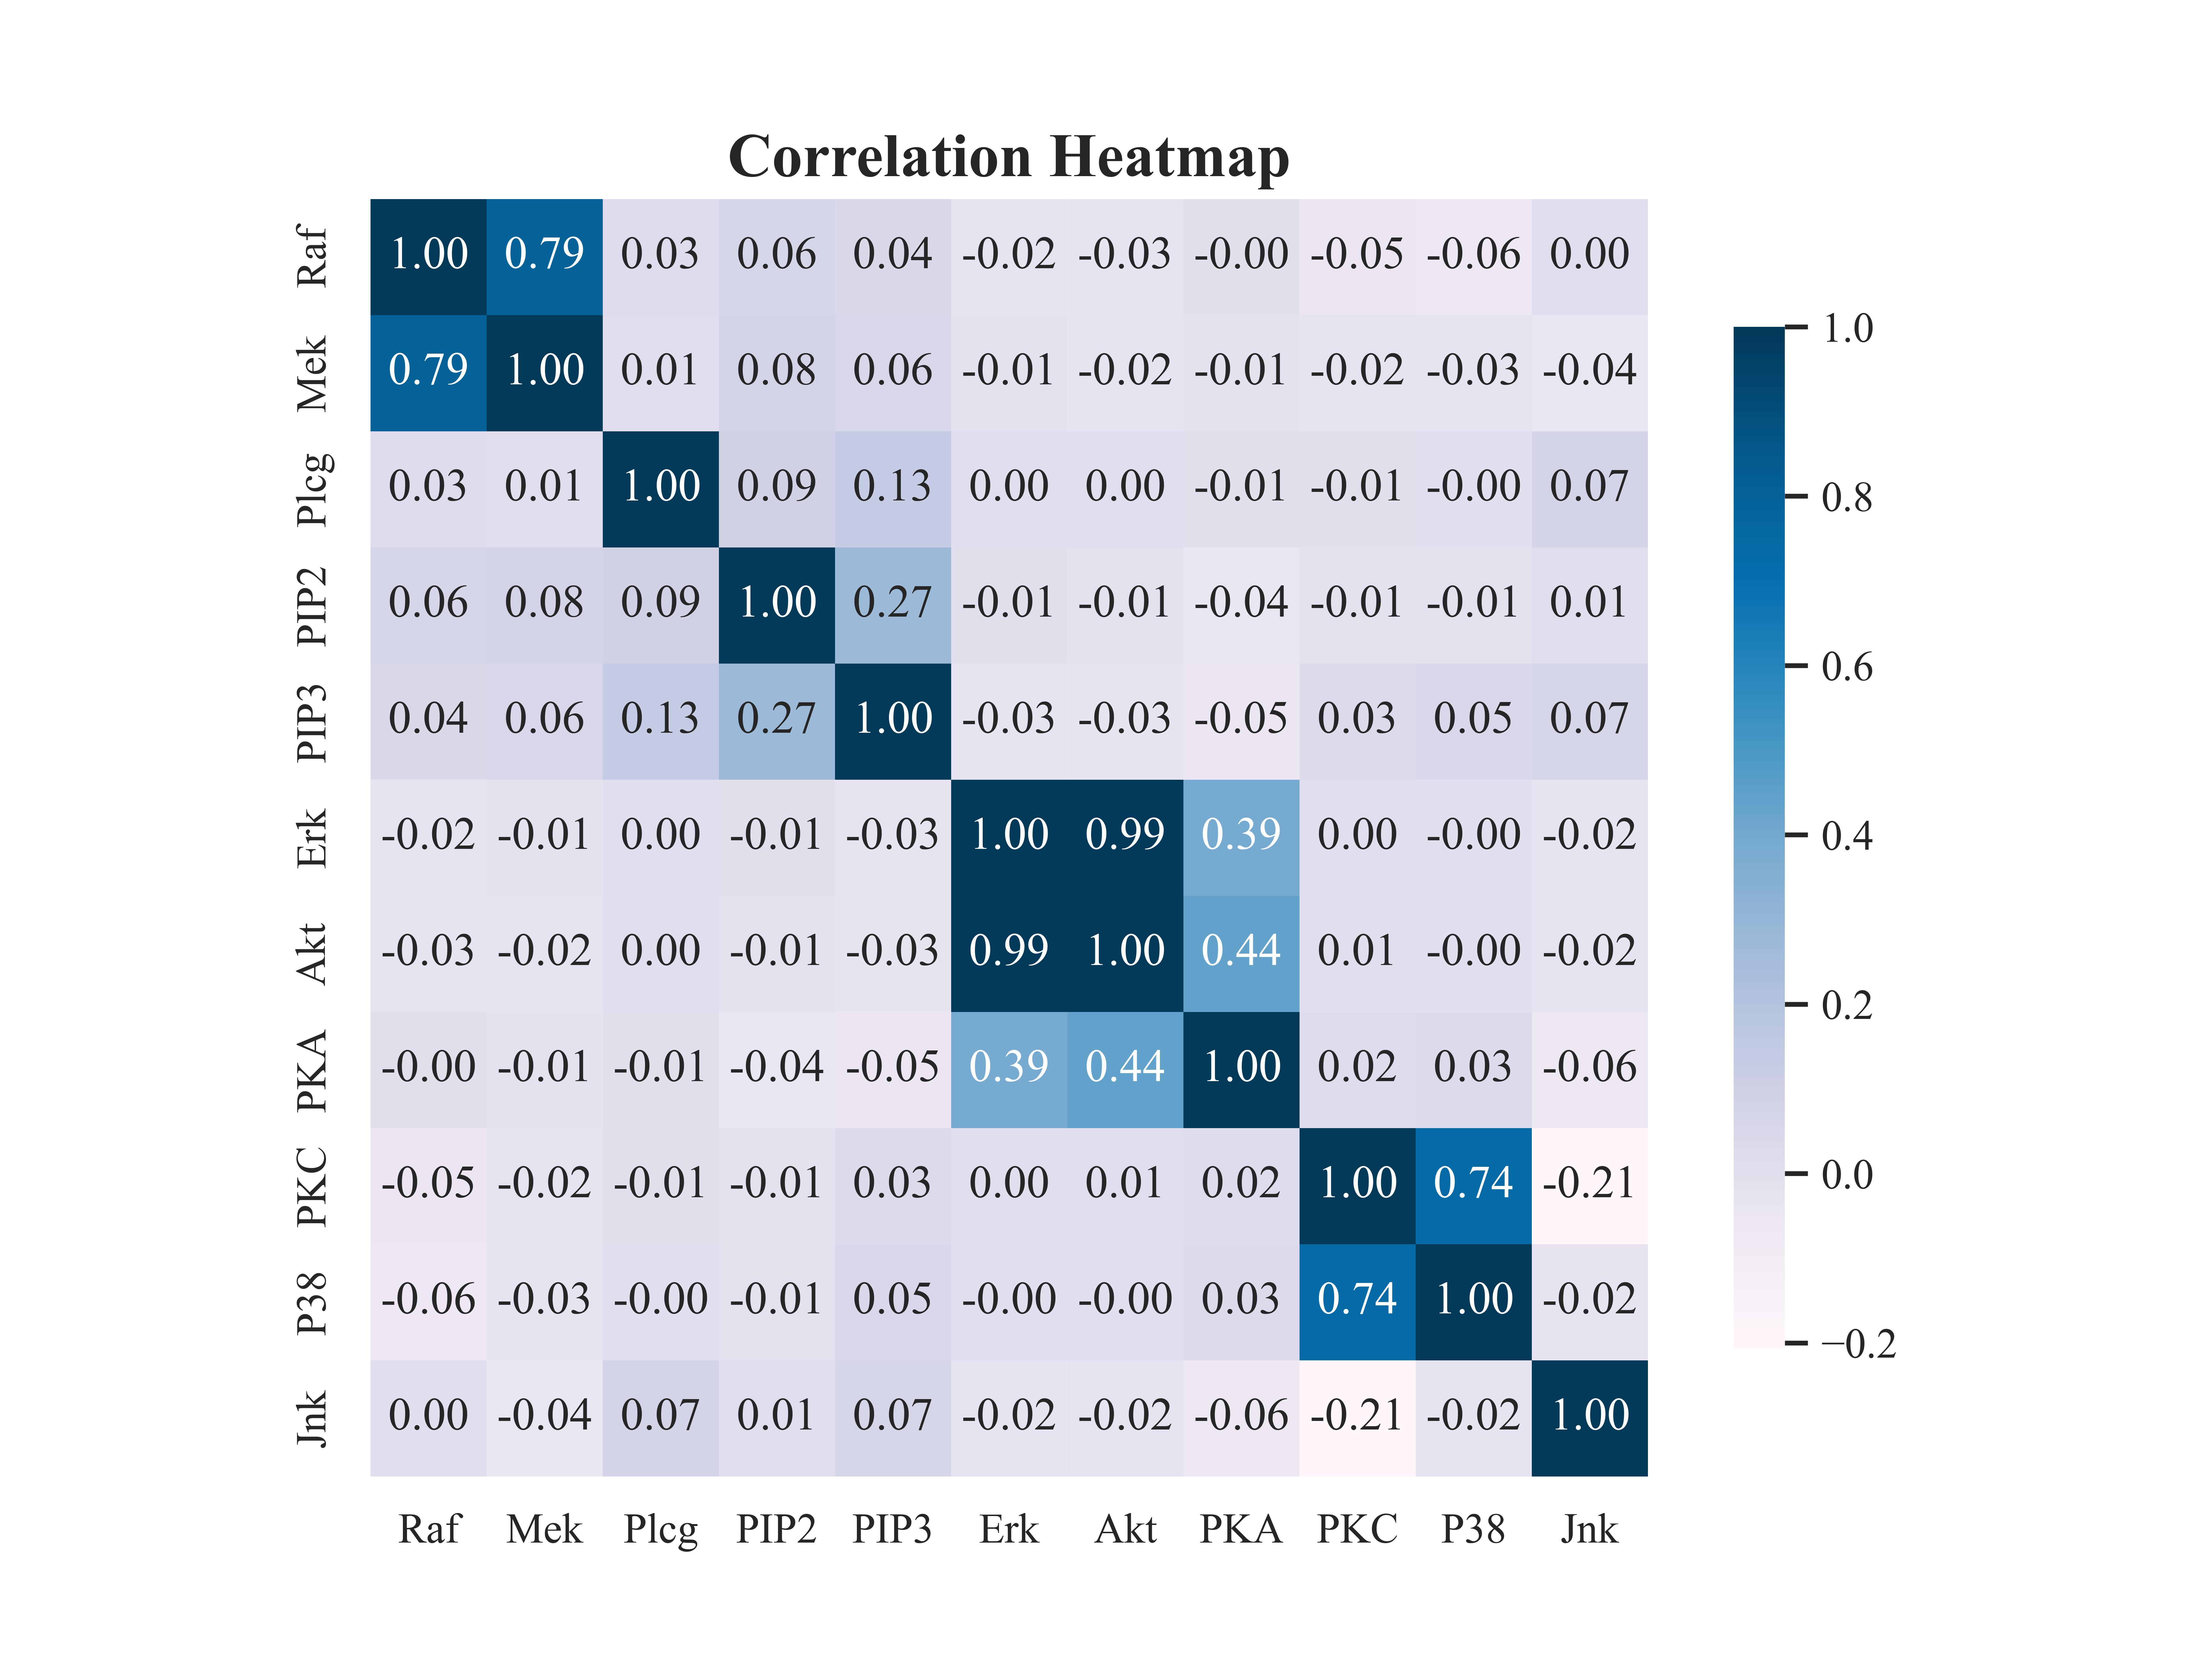
\includegraphics[width=\linewidth]{./demo_data/20241104_133008/sachs/output_graph/eda_corr.jpg}
        \caption{\label{fig:corr}Correlation Heatmap of Variables}
    \end{figure}
\end{minipage}

\section{Discovery Procedure}

In this section, we provide a detailed description of the causal discovery process implemented by Causal Copilot. 
We also provide the chosen algorithms and hyperparameters, along with the justifications for these selections.

\subsection{Data Preprocessing}
In this initial step, we preprocessed the data and examined its statistical characteristics. 
This involved cleaning the data, handling missing values, and performing exploratory data analysis to understand distributions and relationships between variables.
                
\subsection{Algorithm Selection assisted with LLM}
Following data preprocessing, we employed a large language model (LLM) to assist in 
selecting appropriate algorithms for causal discovery based on the statistical characteristics of the dataset and relevant background knowledge. 
The top three chosen algorithms, listed in order of suitability, are as follows:   

\begin{itemize}
    \item \textbf{PC}:
    \begin{itemize}
        \item \textbf{Description}: The PC algorithm is a constraint-based method that learns the structure of a causal graph from data by testing conditional independencies between variables.
        \item \textbf{Justification}: PC is suitable for this dataset due to its large sample size (853) and the fact that there are no missing values. The algorithm effectively handles continuous data without requiring assumptions about the underlying distributions, making it efficient for the current dataset.
    \end{itemize}
                         
    \item \textbf{GES}:
    \begin{itemize}
        \item \textbf{Description}: Greedy Equivalence Search (GES) is a score-based causal discovery algorithm that identifies the optimal causal structure by navigating the space of equivalence classes of Directed Acyclic Graphs (DAGs).
        \item \textbf{Justification}: GES is appropriate since the dataset is large and continuous, allowing for efficient exploration of causal relationships. It also accounts for complex relationships and can work without requiring linearity, despite the data's non-Gaussian errors.
    \end{itemize}
                         
    \item \textbf{NOTEARS}:
    \begin{itemize}
        \item \textbf{Description}: NOTEARS transforms the problem of learning Directed Acyclic Graphs (DAGs) into a continuous optimization problem, offering scalability for large datasets.
        \item \textbf{Justification}: NOTEARS is suitable for this dataset because it can handle high-dimensional data efficiently and is based on continuous optimization rather than combinatorial search methods. Additionally, its flexibility allows it to adapt to non-linear relationships, which aligns with the statistical properties of the dataset.
    \end{itemize}
\end{itemize}

\subsection{Hyperparameter Values Proposal assisted with LLM}
Once the algorithms were selected, the LLM aided in proposing hyperparameters 
for the chosen algorithm, which are specified below:
        
\begin{itemize}
    \item \textbf{alpha}:
    \begin{itemize}
        \item \textbf{Value}: 0.05
        \item \textbf{Explanation}: This value is appropriate given the large sample size (853), where using a standard significance level of 0.05 balances the need for statistical power and the risk of type I error.
    \end{itemize}
                         
    \item \textbf{findep\_test}:
    \begin{itemize}
        \item \textbf{Value}: fisherz
        \item \textbf{Explanation}: Even though the dataset does not follow Gaussian distribution, 'fisherz' is still preferred due to it being the default for continuous data. This choice provides a useful baseline, but caution should be taken due to the non-Gaussian nature of the errors.
    \end{itemize}
                         
    \item \textbf{depth}:
    \begin{itemize}
        \item \textbf{Value}: -1
        \item \textbf{Explanation}: Setting depth to -1 allows for unlimited searching depth. With only 11 variables, this choice facilitates a thorough exploration of dependencies amidst potential nonlinear relationships in the dataset.
    \end{itemize}
\end{itemize}

\subsection{Graph Tuning with Bootstrap and LLM Suggestion}
In the final step, we performed graph tuning with suggestions provided by the Bootstrap and LLM.

Firstly, we use the Bootstrap technique to get how much confidence we have on each edge in the initial graph. If the confidence probability of a certain edge is greater than 95\% and it is not in the initial graph, we force it. Otherwise, if the confidence probability is smaller than 5\% and it exists in the initial graph, we change it to the edge type with the highest probability.

After that, we utilize LLM to help us prune edges and determine the direction of undirected edges according to its knowledge repository. In this step, LLM can use background knowledge to add some edges that are neglected by Statistical Methods. Voting techniques are used to enhance the robustness of results given by LLM, and the results given by LLM should not change results given by Bootstrap.

By integrating insights from both of Bootstrap and LLM to refine the causal graph, we can achieve improvements in graph's accuracy and robustness.

\section{Results Summary}

\subsection{Initial Graph}

\begin{figure}[H]
    \centering
    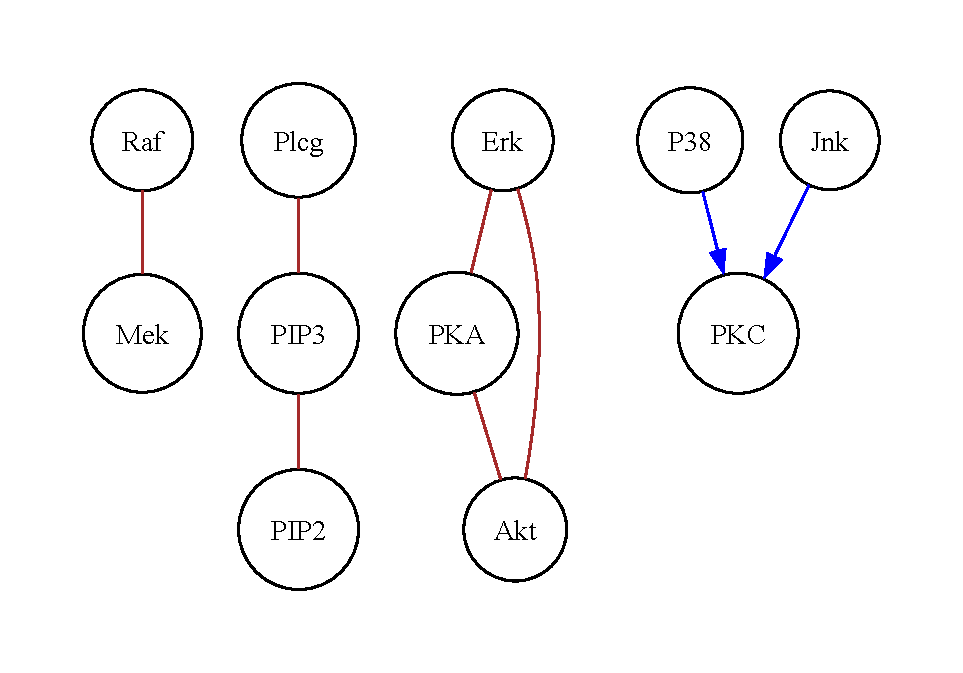
\includegraphics[height=0.3\textheight]{./demo_data/20241104_133008/sachs/output_graph/initial_graph.pdf}
    \caption{Initial Graph}
\end{figure}

The above is the initial result graph produced by our algorithm.

The analysis reveals a complex web of causal interactions among several key signaling proteins. Firstly, Mek has a direct influence on Raf, suggesting that activation of Mek leads to subsequent activation of Raf, which plays a critical role in the MAPK signaling pathway. Furthermore, PIP3, a pivotal lipid second messenger, is impacted by both Plcg and PIP2, indicating that these precursors contribute to the accumulation of PIP3, which in turn can regulate its own precursors, creating a feedback loop. Erk, serving as a crucial mediator in various signaling pathways, shows a bidirectional relationship with both Akt and PKA, illustrating that these proteins mutually influence each other’s activation states, ultimately connecting to various cellular functions such as metabolism and cell growth. Additionally, P38 and Jnk have a causal influence on PKC, further integrating these signaling pathways within cellular stress responses. Overall, this intricate interaction map underscores the dynamic relationships between these signaling molecules, highlighting the complexity of cellular signaling networks.

\subsection{Revised Graph}

\begin{minipage}[t]{0.6\linewidth}
    
By using the method mentioned in the Section 4.4, we provide a revised graph pruned with Bootstrap and LLM suggestion. Pruning results are as follows.
        
The following are force results given by LLM:
            
\begin{itemize}
    
    \item \textbf{Mek $\rightarrow$ Erk}: Mek activates Erk through phosphorylation, making Erk a downstream target of Mek in the MAPK signaling pathway.
    
    \item \textbf{Plcg $\rightarrow$ PIP2}: Plcg hydrolyzes PIP2 to produce inositol trisphosphate and diacylglycerol, directly linking Plcg to the regulation of PIP2 levels in signaling cascades.
    
\end{itemize}
            
The following are directions of remaining undirected edges determined by the LLM:
\begin{itemize}

\item \textbf{Raf $\rightarrow$ Mek}: Raf activates Mek through phosphorylation, playing a crucial role in the MAPK signaling pathway.

\item \textbf{Plcg $\rightarrow$ PIP3}: Phospholipase C-gamma (Plcg) hydrolyzes PIP2, leading to the generation of PIP3, thus creating a direct relationship between these two molecules in the signaling cascades.

\item \textbf{PIP2 $\rightarrow$ PIP3}: PIP2 is a substrate for phospholipase C that is converted into PIP3, establishing PIP2 as a precursor in the pathway leading to the production of PIP3.

\item \textbf{PKA $\rightarrow$ Erk}: While Akt can influence PKA activity indirectly, this relationship is context-dependent; direct activation of Erk involves the MAPK pathway, making the relationship more nuanced.

\end{itemize}
            
This structured approach ensures a comprehensive and methodical analysis of the causal relationships within the dataset.
        
\vfill
\end{minipage}
\hfill
\begin{minipage}[t]{0.4\linewidth}
    \begin{figure}[H]
        \centering
        \vspace{-0.5cm}
        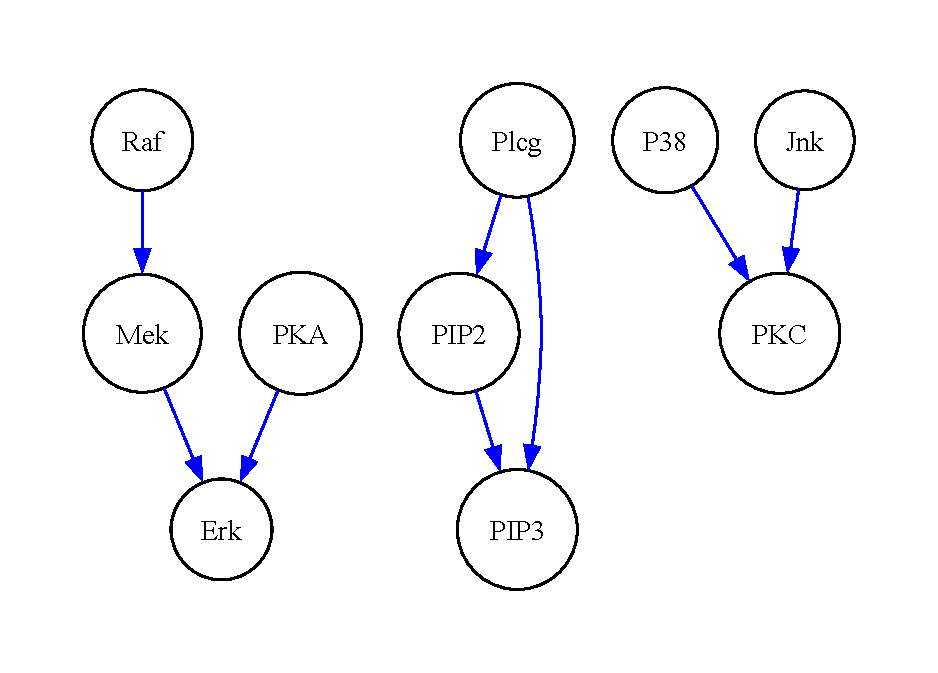
\includegraphics[width=\linewidth]{./demo_data/20241104_133008/sachs/output_graph/revised_graph.pdf}
        \caption{\label{fig:corr}Revised Graph}
    \end{figure}
\end{minipage}

\subsection{Graph Reliability Analysis}

\begin{figure}[H]
    \centering
    \begin{subfigure}{0.32\textwidth}
        \centering
        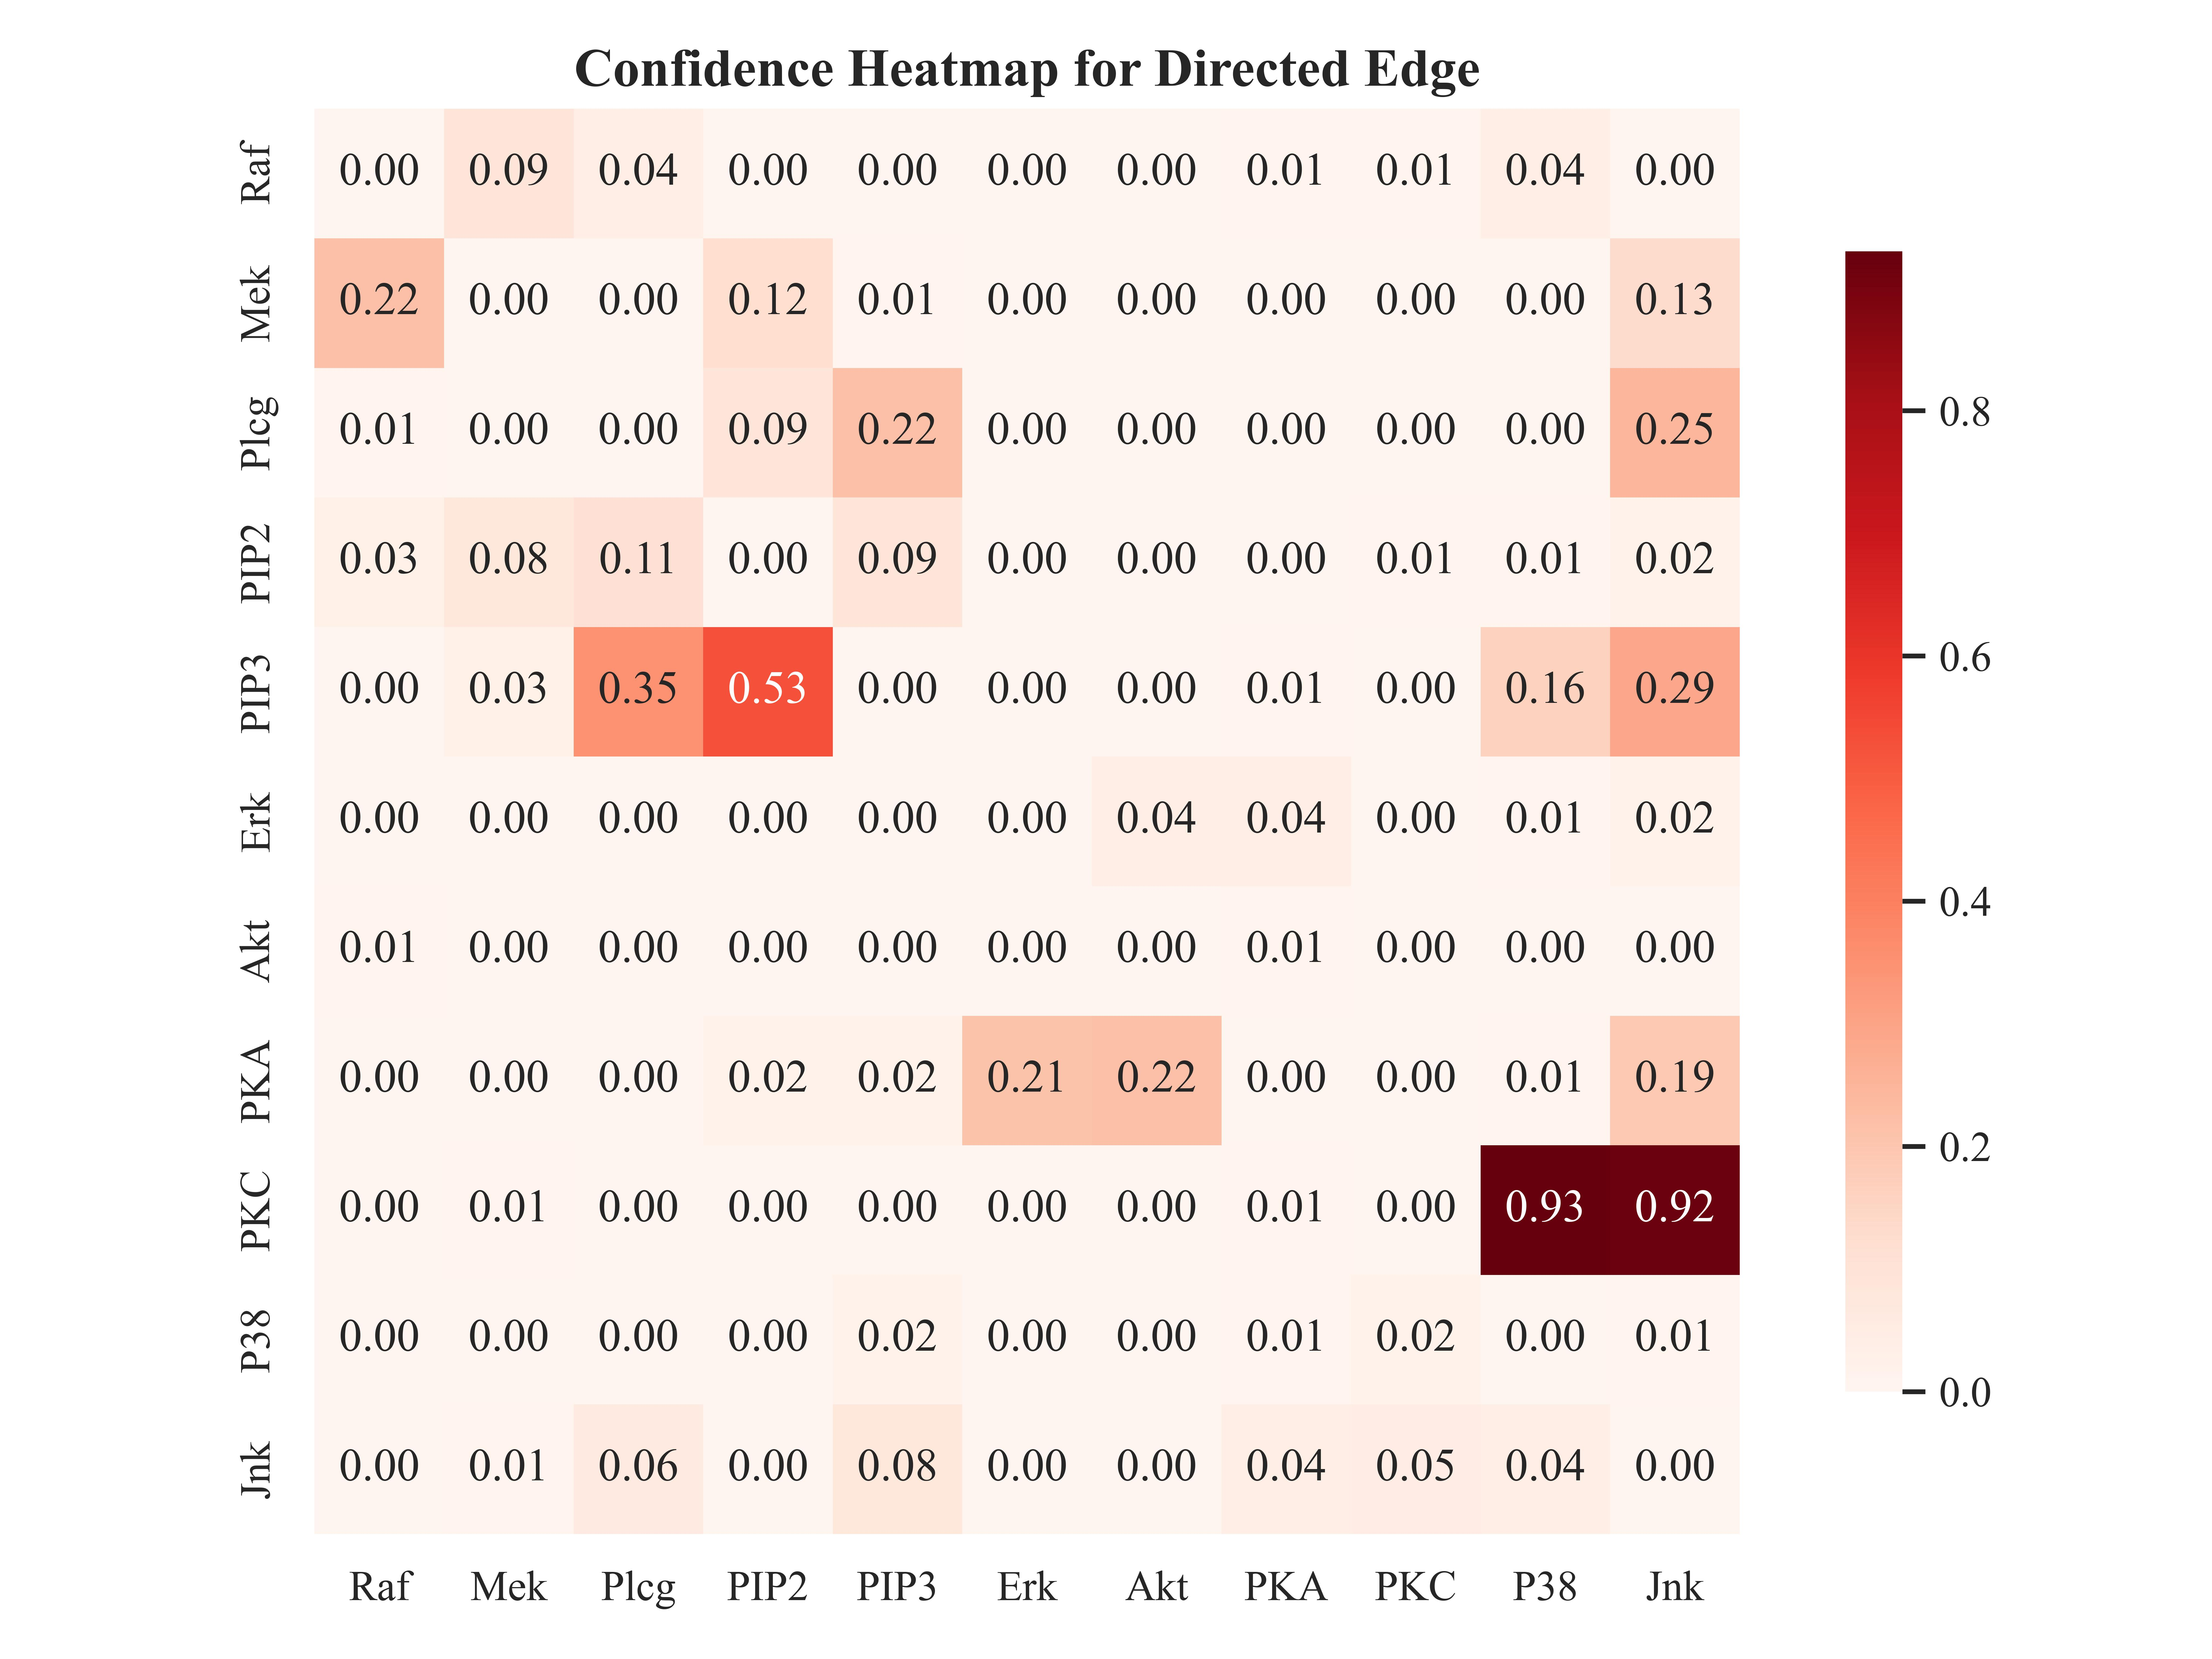
\includegraphics[width=\linewidth]{./demo_data/20241104_133008/sachs/output_graph/certain_edges_confidence_heatmap.jpg}
        \caption{Directed Edge Edge}
    \end{subfigure}
    \begin{subfigure}{0.32\textwidth}
        \centering
        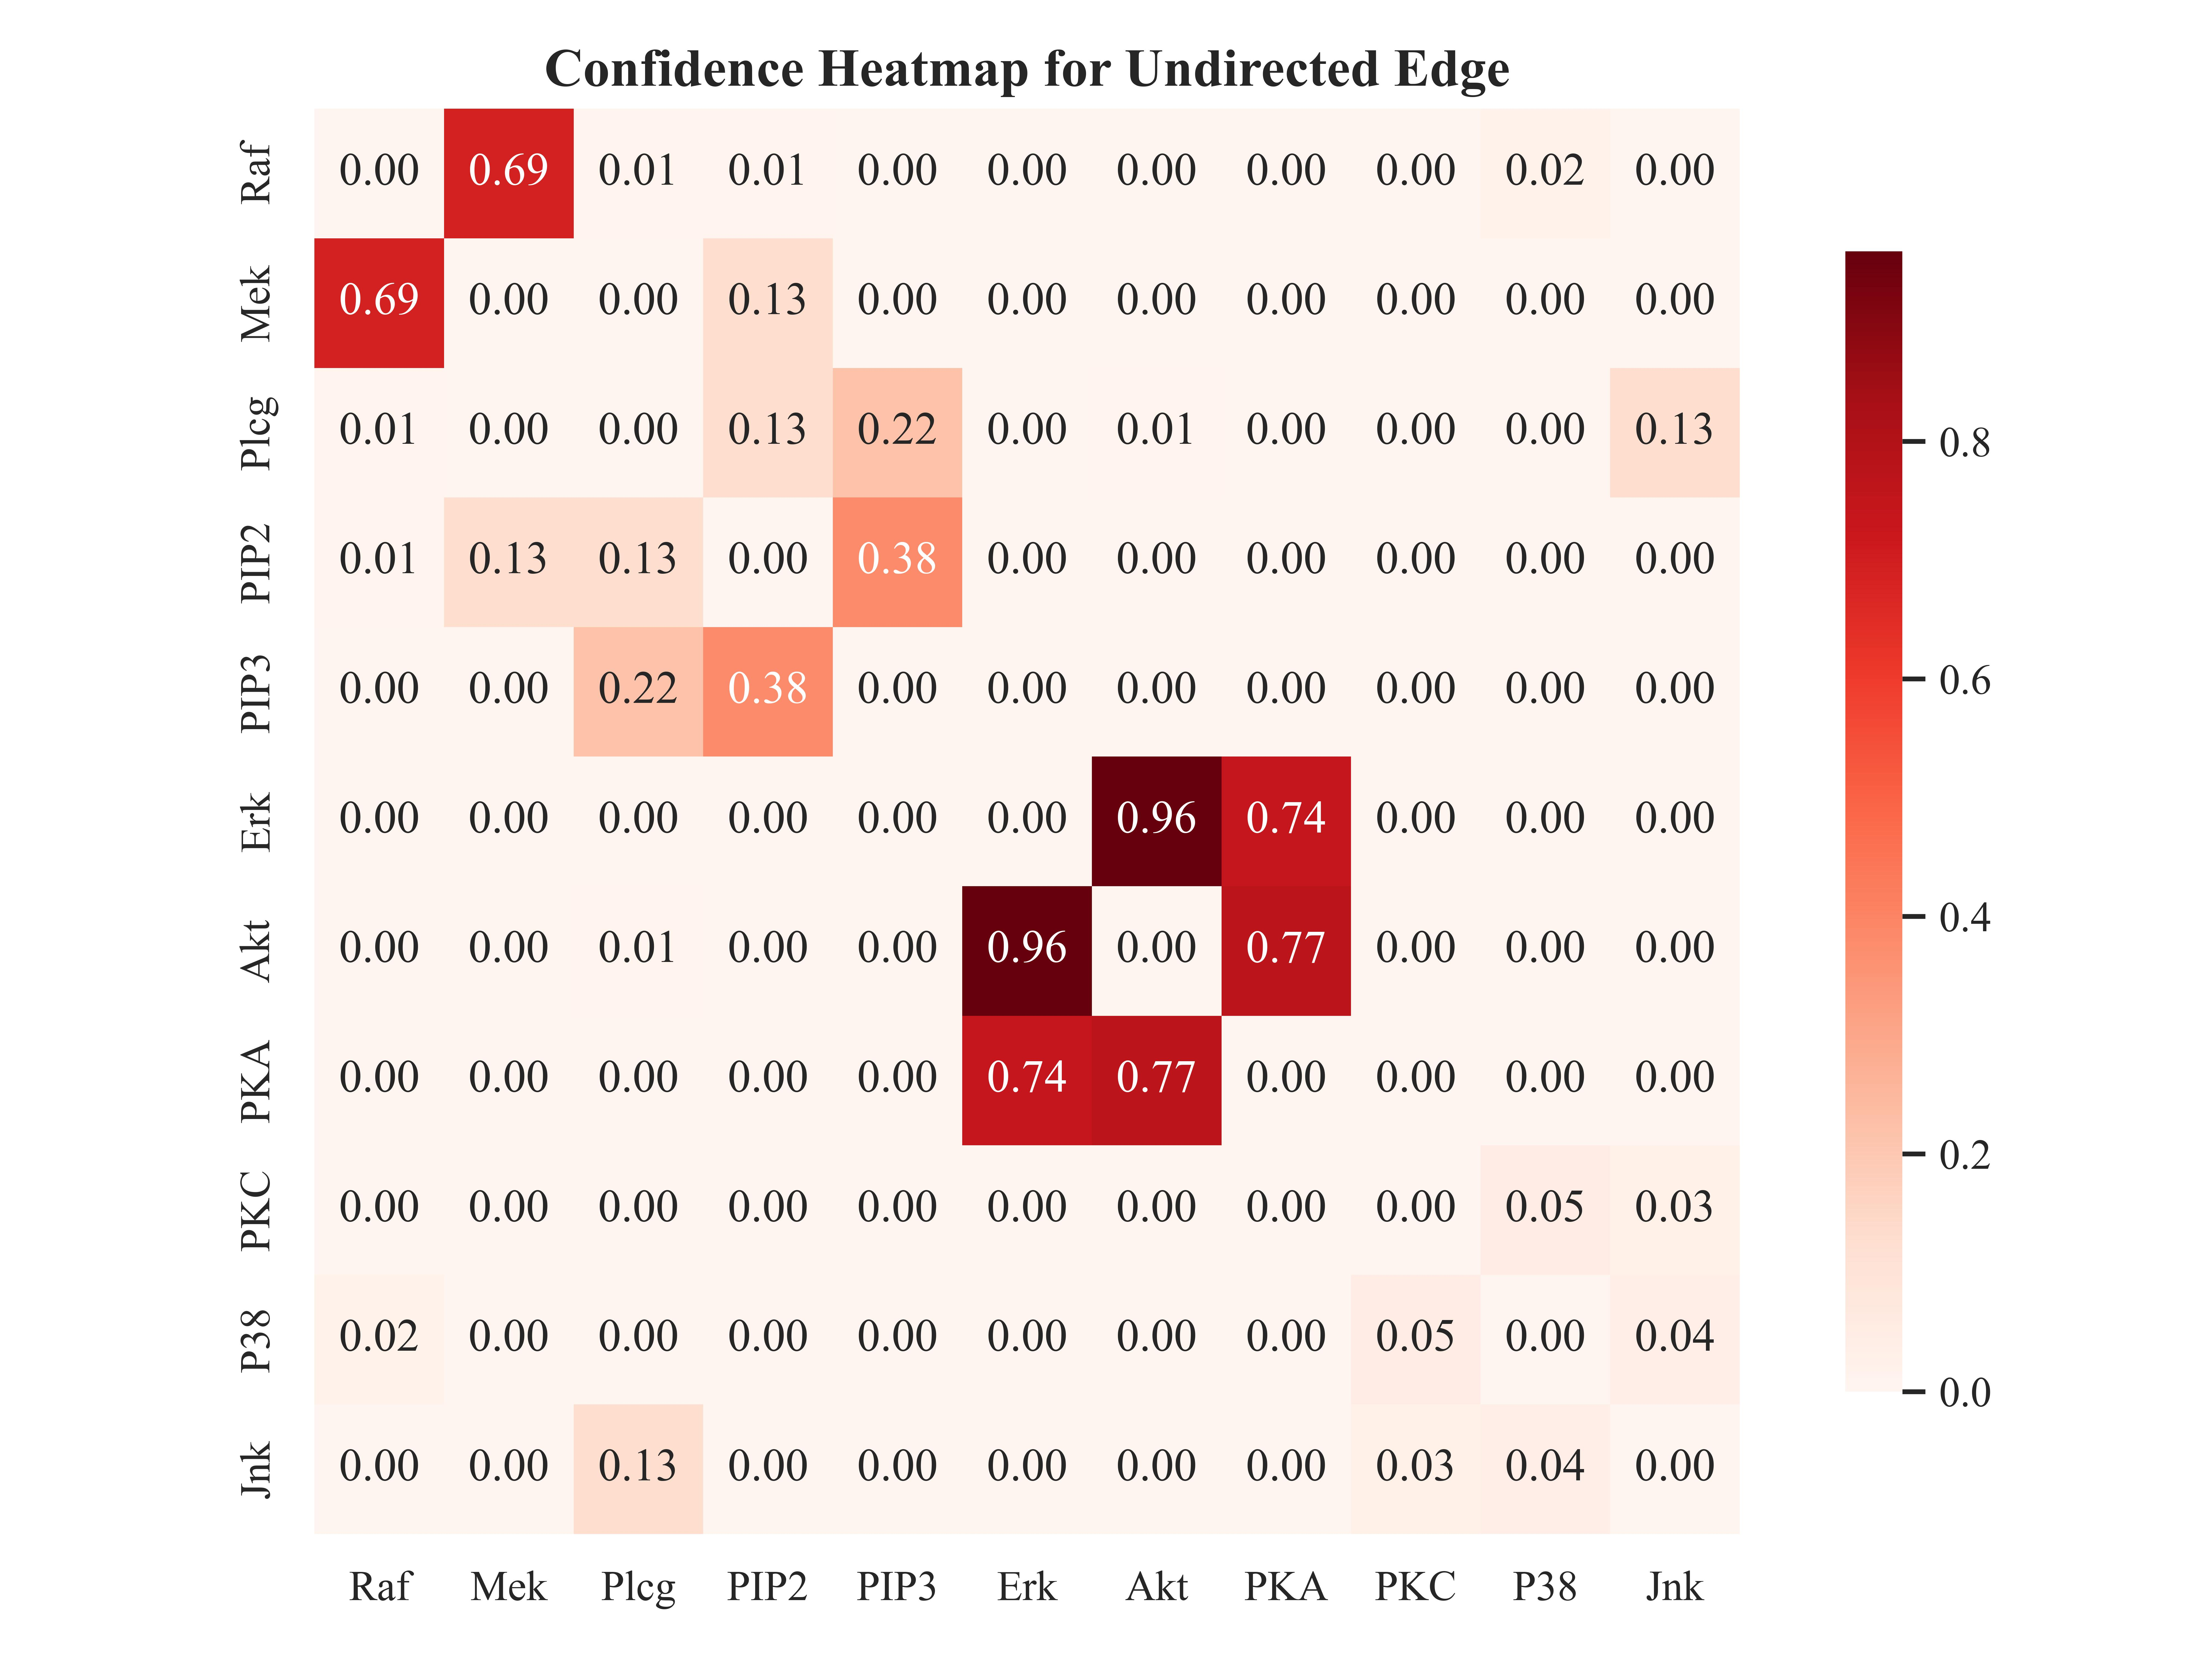
\includegraphics[width=\linewidth]{./demo_data/20241104_133008/sachs/output_graph/uncertain_edges_confidence_heatmap.jpg}
        \caption{Undirected Edge Edge}
    \end{subfigure}
    \begin{subfigure}{0.32\textwidth}
        \centering
        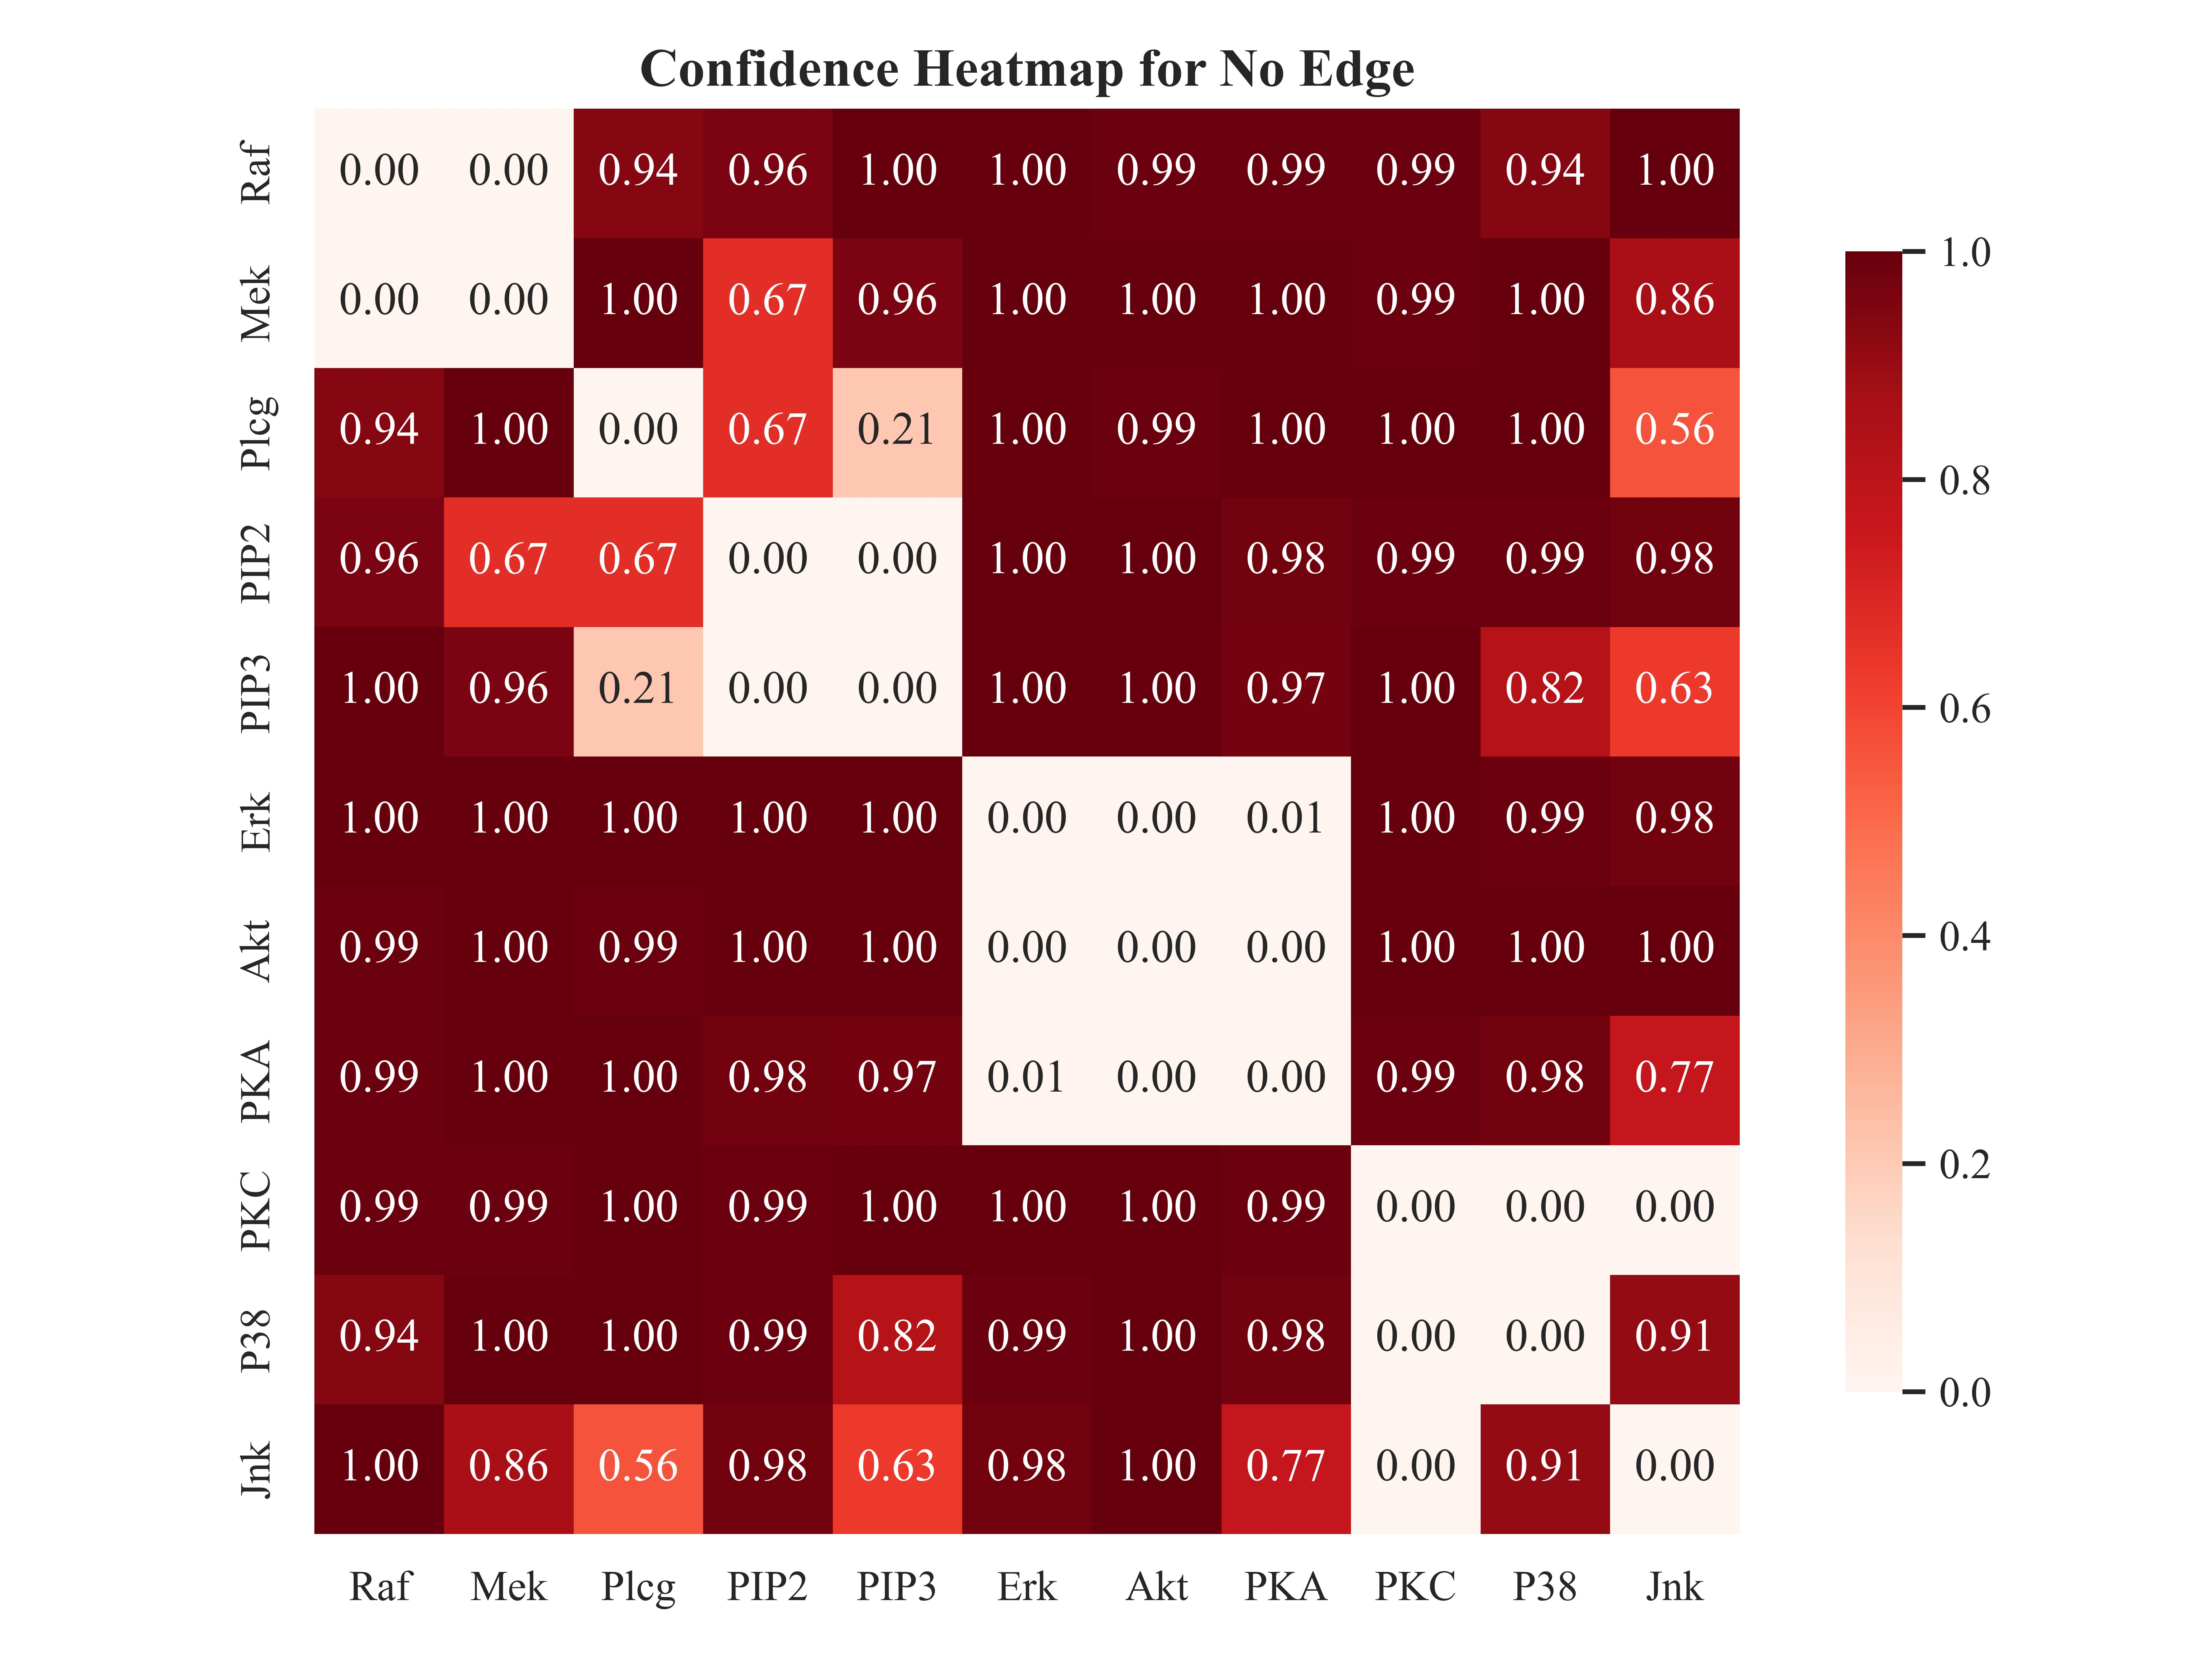
\includegraphics[width=\linewidth]{./demo_data/20241104_133008/sachs/output_graph/non_existence_confidence_heatmap.jpg}
        \caption{No Edge Edge}
    \end{subfigure}
    \caption{Confidence Heatmap of Different Edges}
\end{figure}

The above heatmaps show the confidence probability we have on different kinds of edges, including directed edge ($\rightarrow$), undirected edge ($-$), No Edge, and probability of no edge. The heatmap of bi-edges is not shown because probabilities of all edges are 0. Based on the confidence probability heatmap and background knowledge, we can analyze the reliability of our graph.

From the statistics perspective, we have high confidence to believe that these edges exist: PIP3 $\rightarrow$ PIP2 (bootstrap probability of 0.53) and PIP3 $\rightarrow$ Plcg (0.35), indicating a moderate to high likelihood of these causal relationships. Conversely, we have low confidence in the presence of edges such as Raf $\rightarrow$ Mek (0.09), Erk $\rightarrow$ Akt (0.04), and P38 $\rightarrow$ PKC (0.02), suggesting that the evidence for these relationships is weak. 

However, based on expert knowledge, we know that the edges Raf $\rightarrow$ Mek and Mek $\rightarrow$ Erk represent well-established signaling pathways, while the relationship PIP3 $\rightarrow$ Akt is crucial for Akt activation, suggesting these edges indeed exist despite their low bootstrap probabilities. Additionally, the relationships Erk $\rightarrow$ PKA and P38 $\rightarrow$ PKC are less supported by the known biological interactions, which question their inclusion in the causal graph. 

Therefore, while the results of this causal graph indicate specific pathways that are supported by both statistical evidence and domain knowledge, the low bootstrap probabilities challenge the reliability of certain edges. Consequently, we can conclude that the causal graph has mixed reliability; it is reliable for pathways connecting PIP3, Raf, Mek, and Erk but less so for edges with low statistical confidence and weaker support from expert knowledge.

\end{document}